\documentclass{ctexart}
\usepackage{graphicx}
\usepackage{caption}
\usepackage{float}
\usepackage{amsmath}
\usepackage{fancyhdr}
\usepackage{xunicode-addon}
\usepackage{booktabs}
\usepackage[a4paper,hmargin=1.25in,vmargin=1in]{geometry}
% !TeX program = xelatex
\title{\begin{figure}[H]
	\centering 
	\includegraphics[height=7cm,width=14cm]{E:/Pictures/中科大.jpg}
	\end{figure}\Huge\textbf{Lab 5}\\\huge{三次样条插值}}
\date{}
\punctstyle{banjiao} 
\pagestyle{fancy}
	\fancyhead[C]{\LARGE\textbf{Lab 5}}
	\fancyhead[L]{}
	\fancyhead[R]{}
	\fancyfoot[C]{\thepage}
\begin{document}
	\maketitle
	\thispagestyle{empty}
	
	\[\makebox{\Large{姓名:\underline{\makebox[5cm]{高茂航}}}}\]
	
    \[\makebox{\Large{学号:\underline{\makebox[5cm]{PB22061161}}}}\]
	
	$$\makebox{\Large{日期:\underline{\makebox[5cm]{2024.5.10}}}}$$
	
	\clearpage

	\pagenumbering{arabic}
	\section{Problem Descriptions}
	给定若干插值点,利用大M法计算三次样条插值函数,实现三次样条插值算法。
	\section{Analysis and Algorithms} 
	$$\mu_{i}M_{i-1}+2M_{i}+\lambda_{i}M_{i+1}=d_{i},i=1,2,\cdots,n-1$$

其中

$$\mu_{i}=1-\lambda_{i}$$

$$\frac{h_{i}}{h_{i}+h_{i}}$$

$$d_{i}=\frac{6}{h_{i}+h_{i-1}}\left({\frac{y_{i+1}-y_{i}}{h_{i}}-\frac{y_{i}-y_{i-1}}{h_{i-1}}}\right)=6f\left(x_{i-1},x_{i},x_{i+1}\right)$$

给 定  $M_{0}, M_{n}$的值,此时$n-1$个方程组有$n-1$个未知量$\left\{M_i,i=1,2,\cdots,n-1\right\}$.当$M_{0}=0,M_{n}=0$时,称为自然边界条件.
$$\begin{bmatrix}2&\lambda_{1}\\\mu_{2}&2&\lambda_{2}\\&\ddots&\ddots&\ddots\\&&\mu_{n-2}&2&\lambda_{n-2}\\&&&\mu_{n-1}&2\end{bmatrix}\begin{bmatrix}M_{1}\\M_{2}\\\\M_{n-2}\\\\M_{n-1}\end{bmatrix}=\begin{bmatrix}d_{1}-\mu_{1}M_{0}\\d_{2}\\\vdots\\d_{n-2}\\d_{n-1}-\lambda_{n-1}M_{n}\end{bmatrix}$$
$$\begin{aligned}S\left(x\right)=&\frac{\left(x_{i+1}-x\right)^{3}M_{i}+\left(x-x_{i}\right)^{3}M_{i+1}}{6h_{i}}+\frac{\left(x_{i+1}-x\right)y_{i}+\left(x-x_{i}\right)y_{i+1}}{h_{i}}\\&-\frac{h_{i}}{6}[(x_{i+1}-x)M_{i}+(x-x_{i})M_{i+1}],\quad x\in[x_{i},x_{i+1}]\end{aligned}$$
	\section{Results}
		
	\begin{figure}[H]
		\centering 
		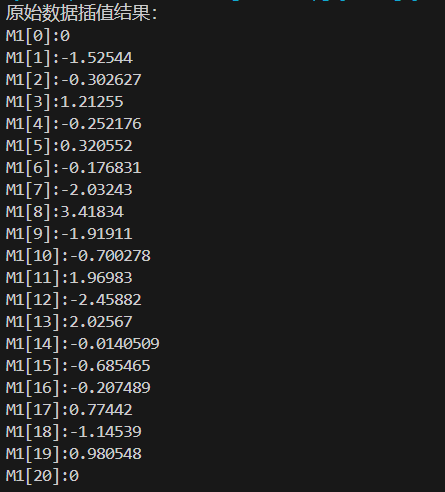
\includegraphics[height=8cm,width=7cm]{1.png}
		\end{figure}
		\begin{figure}[H]
			\centering 
			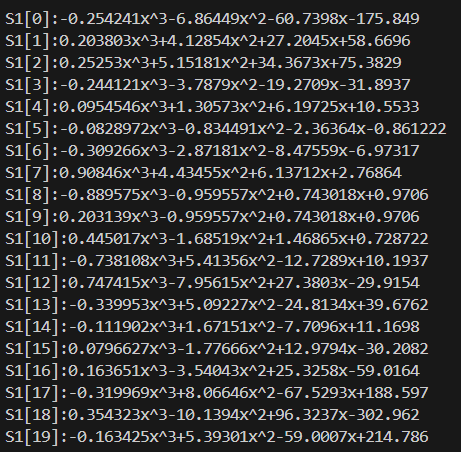
\includegraphics[height=8cm,width=7cm]{2.png}
			\end{figure}
			\begin{figure}[H]
				\centering 
				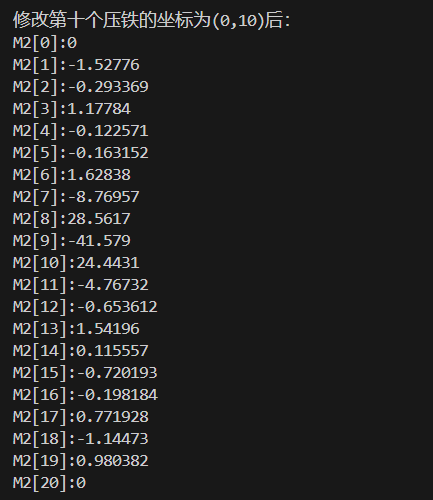
\includegraphics[height=8cm,width=7cm]{3.png}
				\end{figure}
				\begin{figure}[H]
					\centering 
					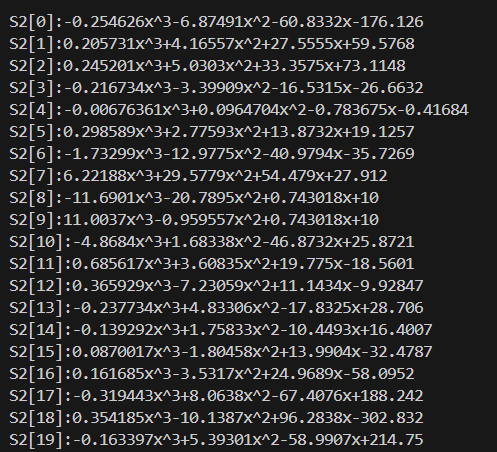
\includegraphics[height=8cm,width=7cm]{4.png}
					\end{figure}
		\section{Conclusion}
		在各个多项式中入相应插值点的值,发现曲线能较准确地拟合。将第十个点的坐标改为(0,10)后,计算出新的曲线中M值都改变了,每个区间内的三次函数也都发生了改变。
    \end{document}